\documentclass[12pt, a4paper]{article}
\usepackage[margin=1in, bottom=1.6in]{geometry}

% Links
\usepackage{hyperref}

\usepackage{booktabs} % Table
% \usepackage[tableposition=top]{caption} % captions?
\usepackage{caption}
\usepackage{enumitem} % Itemize letters

% picture-y packages
\usepackage{graphicx} % Include images
\usepackage{placeins} % For \FloatBarrier
\usepackage[dvipsnames]{xcolor} 
\usepackage{xcolor} 
\usepackage{tikz}
\usetikzlibrary{positioning}
\usepackage{adjustbox}

% math packages
\usepackage{textcomp} % For the \degree command
\usepackage{amsmath}  % Include the amsmath package
\usepackage{siunitx}
\usepackage{pgf} % Math Calculations
\usepgflibrary{fpu} % To process large numbers
\pgfkeys{
    /pgf/fpu = true,
    /pgf/number format/.cd,
    precision=2,
    fixed,
    fixed zerofill,
    use comma,
    1000 sep={.}
}

% For degree symbol
\usepackage[utf8]{inputenc}
\usepackage[T1]{fontenc}
\usepackage{textcomp}
\usepackage{gensymb}

% Adding code to report
\usepackage{listings}
\usepackage{color}

\definecolor{dkgreen}{rgb}{0,0.6,0}
\definecolor{gray}{rgb}{0.5,0.5,0.5}
\definecolor{mauve}{rgb}{0.58,0,0.82}

\lstset{frame=tb,
  language=Java,
  aboveskip=3mm,
  belowskip=3mm,
  showstringspaces=false,
  columns=flexible,
  basicstyle={\small\ttfamily},
  numbers=none,
  numberstyle=\tiny\color{gray},
  keywordstyle=\color{blue},
  commentstyle=\color{dkgreen},
  stringstyle=\color{mauve},
  breaklines=true,
  breakatwhitespace=true,
  tabsize=3
}

\begin{document}
\title{Model of Flight Path and Arm}
\author{George D}
\maketitle{}

\section{DELIVERABLES}

\subsection{Deliverable A}

\textbf{Given the flight path $y(x) = \sqrt{100-x}$, derive the expressions for the radius of curvature, $\rho$, and the basis vectors $\hat{e_t}$, $\hat{e_n}$ of the tangential/normal coordinate system as functions of x of the flight path. For the basis vectors, express your results in the xy coordinate system: $\hat{e_t} = e_{tx}\hat{i} + e_{ty}\hat{j}$ and $\hat{e_n} = e_{nx}\hat{i} + e_{ny}\hat{j}$.} \\

Taking the derivative and second derivative of the function that describes the flight path:

\begin{equation}
    y' = - \frac{1}{2\sqrt{100-x}}
\end{equation}

\begin{equation}
    y" = - \frac{1}{4(100-x)^\frac{3}{2}}
\end{equation}

The radius of curvature $\rho$ is given by the following equation: 

\begin{equation}
    \rho = |\frac{(1 + y'^2)^\frac{3}{2}}{y"}| \\ 
\end{equation}

This radius can be expressed as a function of x by replacing y' and y" in equation 3 by equations 1 and 2.

\begin{align*}
    \rho = |\frac{(1 + (- \frac{1}{2\sqrt{100-x}})^2)^\frac{3}{2}}{- \frac{1}{4(100-x)^\frac{3}{2}}}| \\ 
    \rho = - \frac{-(4x+401)^{3/2} \cdot 4(100-x)^{3/2}}{8(100-x)^{3/2} \cdot 1} \\ 
\end{align*}
\begin{equation}
    \rho = - \frac{(-4x+401)^{\frac{3}{2}}}{2}
\end{equation}

The function for the flight path may be described in terms of the basis vectors $\hat{e_t}$, $\hat{e_n}$ or in the xy coordinate system. Figure 1 describes the flight path of the NFC.

\begin{figure}[htbp]
    \centering
    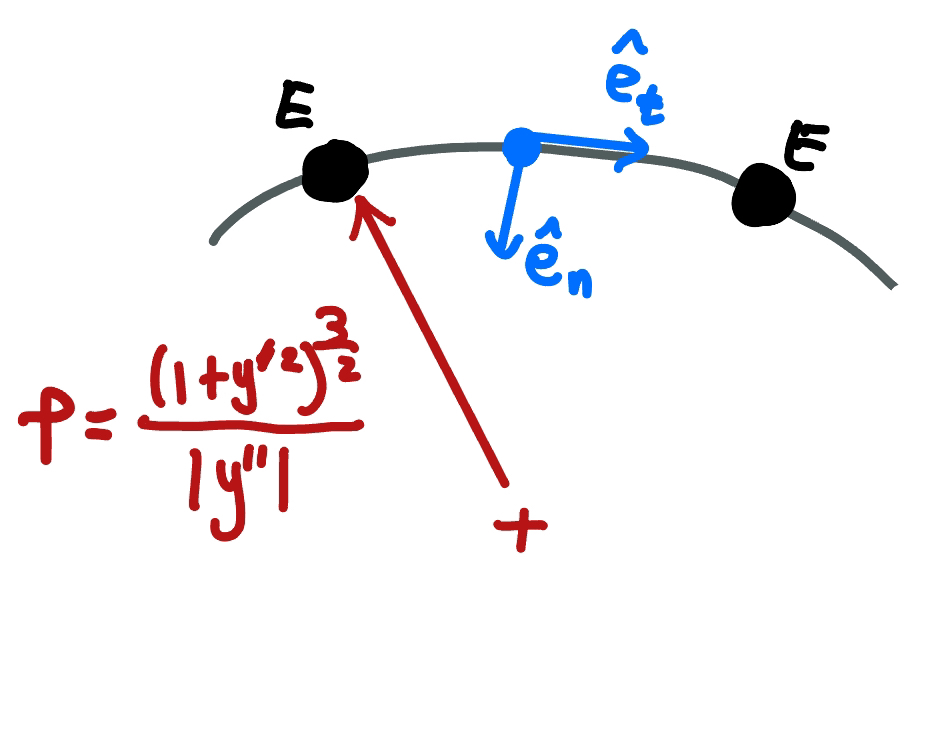
\includegraphics[width=0.3\textwidth]{figure1.jpeg}
    \caption{Tangential/Normal Coordinate System}
    \label{fig:label2}
\end{figure}

The derivative of the function of the flight path can give information on the direction of the NFC. The tangent unit vector points along the tangent of the curve. \\

To represent the direction of $\hat{e_t}$ in the xy-system, we use the expression $\frac{(1, y')}{\sqrt{1^2+(y')^2}}$. 1 represents the direction along the x-axis, and y' represents the slope of the tangent. Additionally, $\hat{e_n}$ can be represented by $\frac{(y', 1)}{\sqrt{(y')^2+1^2}}$, the "1" representing the change in the y-direction and its perpendicular direction with respect to the tangential vector, as well as the slope of the tangent again. These values can be expressed as functions of x: 

\begin{equation}
    \hat{e_t} = \frac{(1, y')}{\sqrt{1^2+(y')^2}} = (\frac{1}{\sqrt{1^2+(- \frac{1}{2\sqrt{100-x}})^2}}, \frac{- \frac{1}{2\sqrt{100-x}}}{\sqrt{1^2+(- \frac{1}{2\sqrt{100-x}})^2}})
\end{equation}

\begin{equation}
    \hat{e_n} = \frac{(y', 1)}{\sqrt{(y')^2+1^2}} = (\frac{- \frac{1}{2\sqrt{100-x}}}{\sqrt{1^2+(- \frac{1}{2\sqrt{100-x}})^2}}, \frac{1}{\sqrt{1^2+(- \frac{1}{2\sqrt{100-x}})^2}})
\end{equation}

To simplify the equations further, we have: 

\begin{equation}
    \hat{e_t} = (\frac{2\sqrt{100-x}}{\sqrt{-4x+401}}, \frac{-1}{\sqrt{-4x+401}}) = (\frac{2\sqrt{100-x}}{\sqrt{-4x+401}})\hat{i} + (\frac{-1}{\sqrt{-4x+401}})\hat{j}
\end{equation}

\begin{equation}
    \hat{e_n} = (\frac{1}{\sqrt{-4x+401}},\frac{2\sqrt{100-x}}{\sqrt{-4x+401}}) = (\frac{1}{\sqrt{-4x+401}})\hat{i} + (\frac{2\sqrt{100-x}}{\sqrt{-4x+401}})\hat{j}
\end{equation}

\newpage
\subsection{Deliverable B}

\textbf{Let the NFC velocity and acceleration be $\vec{V_{NFC}}\hat{e_t}$ and $\vec{a_{NFC}} = a_{t NFC}\hat{e_t}+a_{n NFC}\hat{e_n}$. Given $\vec{V_{E1}} = 4\hat{e_t}$, and the constant deceleration ($a_{t NFC}$ = constant), write down the expressions for $V_{NFC}, a_{n NFC}$ as functions of the distance traveled along the flight path. Note the motion of NFC matches exactly the motion of point E of the reach arm.} \\ \\ 

Let $\Delta s$ represent the distance traveled along the flight path.

A small change in the motion of the NFC can be described as the following: 

\begin{equation}
    ds = (\sqrt{1^2+(\frac{dy}{dx})^2})dx
\end{equation}

To get the total distance traveled to a certain point x, integration can be performed: 

\begin{equation}
    \Delta s = \int_{0}^{x} \sqrt{1^2+(\frac{dy}{dx})^2} \, dx = \int_{0}^{x} \sqrt{1^2+(- \frac{1}{2\sqrt{100-x}})^2} \, dx
\end{equation}

To describe the motion of a particle moving along a certain path, such as the NFC, the following equation can be used, where $a$ is the constant acceleration:

\begin{equation}
    V_{\text{final}}^2 = V_{\text{initial}}^2 + 2\cdot{\text{a}}\cdot\Delta{\text{s}}
\end{equation}

Replacing these general variables for the ones in equation for this problem, where $V_{NFC} = V_{E}$ as the motion of NFC matches exactly the motion of point E of the reach arm. 

\begin{equation}
    V_{\text{E2}}^2 = V_{E1}^2 - 2 \cdot a_{\text{t NFC}}\cdot \Delta s
\end{equation}

Or simplified to the equation below ($\vec{V_{E1}} = 4\hat{e_t}$) and the speed of the NFC solved for:

\begin{equation}
    V_{\text{NFC}} = \sqrt{4^2 - 2 \cdot a_{\text{t NFC}}\cdot s}
\end{equation}

\begin{equation}
    V_{\text{NFC}} = \sqrt{16 - 2 \cdot a_{\text{t NFC}}\cdot \Delta s}
\end{equation}

The value of $a_t$ is equal to the expression below.

\begin{equation}
    a_t = \frac{\Delta V_{NFC}}{\Delta t}
\end{equation}

However, since there is \textbf{constant deceleration}, 

\begin{equation}
    a_t = 0
\end{equation}

The normal acceleration of a particle moving along a path is given by $\frac{V^2}{\rho}$. This formula can be modified for the variables of interest in this lab:

\begin{equation}
    a_{\text{n NFC}} = \frac{V_{NFC}^2}{\rho} \hat{e_n}
\end{equation}

\newpage
\subsection{Deliverable C}

\textbf{Let the angular velocities and acceleration of the base arm CD be $\vec{\omega_{CD}}=\dot\phi \hat{k}$, $\vec{a_{CD}}=\ddot\phi \hat{k}$ and the angular velocity and acceleration of the reach arm DE be $\vec{\omega_{DE}}=\dot\theta \hat{k}$, $\vec{a_{DE}}=\ddot\theta \hat{k}$, respectively. Also, let the velocity and acceleration of C of the base arm, $\vec{v_c} = V_{cx}\hat{i}$, $\vec{a_c} = a_{cx}\hat{i}$. Use the relative motion analysis to write down, respectively, the GENERAL expressions for velocity and acceleration vectors $\vec{v_E} = V_{Ex}\hat{i} + V_{Ey}\hat{j}$ and $\vec{a_E} = a_{Ex}\hat{i} + a_{Ey}\hat{j}$ in terms of $\dot\phi, \dot\theta, \ddot\phi, \ddot\theta, V_{cx}, a_{cx}$ along with other geometrical parameters.} \\

Based on the two points that can move in this system, the two relative motion equations are:

\begin{align}
    \vec{V_E} = \vec{V_D} + \vec{V_{E/D}} \\
    \vec{a_E} = \vec{a_D} + \vec{a_{E/D}}
\end{align}

\begin{align}
    \vec{V_D} = \vec{V_C} + \vec{V_{D/C}} \\
    \vec{a_D} = \vec{a_C} + \vec{a_{D/C}}
\end{align}

\begin{figure}[htbp]
    \centering
    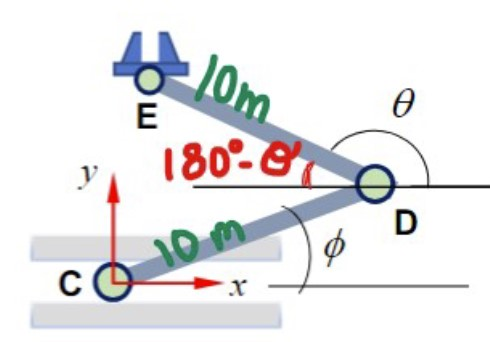
\includegraphics[width=0.3\textwidth]{figure2.jpg}
    \caption{Geometrical Diagram of System}
    \label{fig:label2}
\end{figure}

\FloatBarrier

To obtain the equations for $\vec{r_{D/C}}, \vec{r_{E/D}}$, the diagram in Figure 2 with the angle relationships shown give the following equations and using the origin indicated in Figure 2:

\begin{equation}
    \vec{r_{D/C}} = 10cos\phi\hat{i} + 10sin\phi\hat{j}
\end{equation}

\begin{equation}
    \vec{r_{E/D}} = -10cos(180\degree - \theta)\hat{i} + 10sin(180\degree - \theta)\hat{j}
\end{equation}

\begin{equation}
    \vec{r_{E/D}} = 10cos(\theta)\hat{i} + 10sin(\theta)\hat{j}
\end{equation}

The angular velocity and acceleration dependent on $r$, which can be found in terms of $\theta, \phi$. This can be seen in Figure 2. In general, the velocity of D with respect to C or E to D is $\vec{\omega} \times \vec{r}$. Also, there is no the velocity (so, no acceleration) in the y-direction for C.

\begin{align}
    \vec{V_E} = \vec{V_C} + \vec{V_{D/C}} + \vec{V_{E/D}} \\ 
    \vec{V_E} = \vec{V_{Cx}} + (\vec{\omega_{CD}} \times \vec{r_{D/C}}) + (\vec{\omega_{DE}} \times \vec{r_{E/D}}) \\ 
    \vec{V_E} = \vec{V_{Cx}} + (\dot\phi\hat{k} \times \vec{r_{D/C}}) + (\dot\theta\hat{k} \times \vec{r_{E/D}}) \\ 
    \vec{V_E} = \vec{V_{Cx}} + (\dot\phi\hat{k} \times (10cos\phi\hat{i} + 10sin\phi\hat{j})) + (\dot\theta\hat{k} \times (10cos\theta\hat{i} + 10sin\theta\hat{j}))
\end{align}

Similar is done for the accelerations: 

\begin{align}
    \vec{a_E} = \vec{a_C} + \vec{a_{D/C}} + \vec{a_{E/D}} \\ 
    \vec{a_E} = \vec{a_C} + ((\vec{\alpha_{CD}} \times \vec{r_{C/D}}) + \vec{\omega_{CD}}\times(\vec{\omega_{CD}} \times \vec{r_{D/C}})) + ((\vec{\alpha_{DE}} \times \vec{r_{E/D}}) + \vec{\omega_{DE}}\times(\vec{\omega_{DE}} \times \vec{r_{E/D}})) \\
    \vec{a_E} = \vec{a_C} + ((\ddot\phi\hat{k} \times \vec{r_{C/D}}) + \dot\phi\hat{k} \times(\dot\phi\hat{k} \times \vec{r_{D/C}})) + ((\ddot\theta\hat{k} \times \vec{r_{E/D}}) + \dot\theta\hat{k} \times(\dot\theta\hat{k} \times \vec{r_{E/D}}))
\end{align}

After performing the matrix operations, and replacing the respective values of $r$ within equation 26 (which is not shown because it is a long equation):

\begin{equation}
    \vec{V_E} = [\vec{V_{Cx}}-\dot\phi10sin\phi-\dot\theta10sin\theta]\hat{i} + [\dot\phi10cos\phi + \dot\theta10cos\theta]\hat{j}
\end{equation}

\begin{equation}
    \vec{a_E} = [\vec{a_{Cx}}-\ddot\phi 10sin\phi - \dot\phi^2 10cos\phi - \ddot\theta 10sin\theta - \dot\theta^2 10cos\theta]\hat{i} + [\ddot\phi 10cos\phi - \dot\phi^2 10sin\phi + \ddot\theta 10cos\theta - \dot\theta^2 10sin\theta]\hat{j}
\end{equation}

\newpage
\subsection{Deliverable D}

\textbf{For the capture based on the reach arm DE in translation ($\dot\theta=0, \ddot\theta=0$), simplify the expressions you have in C and write down the expressions in $\phi, \dot\phi, \ddot\phi$}. 

Rewriting the equations 27 and 28, considering $\dot\theta=0, \ddot\theta=0$, the new equations of motion are presented: 

\begin{equation}
    \vec{V_E} = [\vec{V_{Cx}}-\dot\phi10sin\phi]\hat{i} + [\dot\phi10cos\phi]\hat{j}
\end{equation}

\begin{equation}
    \vec{a_E} = [\vec{a_{Cx}}-\ddot\phi 10sin\phi - \dot\phi^2 10cos\phi]\hat{i} + [\ddot\phi 10cos\phi - \dot\phi^2 10sin\phi]\hat{j}
\end{equation}

\newpage
\subsection{Deliverable E}

\textbf{Based on your answers in D, write down the expressions for $V_{cx}$ and $a_{cx}$.}

Rearranging 29 and 30 in terms of $V_{cx}$ and $a_{cx}$: 

\begin{align*}
    \vec{V_{Ex}} = [\vec{V_{Cx}}-\dot\phi10sin\phi]\hat{i} 
\end{align*}

\begin{equation}
    \vec{V_{Cx}} = \vec{V_{Ex}} + \dot\phi10sin\phi
\end{equation}

\begin{align*}
    \vec{a_{Ex}} = [\vec{a_{Cx}}-\ddot\phi 10sin\phi - \dot\phi^2 10cos\phi]\hat{i} 
\end{align*}

\begin{equation}
    \vec{a_{Cx}} = \vec{a_{Ex}} + \ddot\phi 10sin\phi + \dot\phi^2 10cos\phi
\end{equation}

\newpage
\subsection{Deliverable F Part 1, MATLAB Code}

\begin{figure}[htbp]
    \centering
    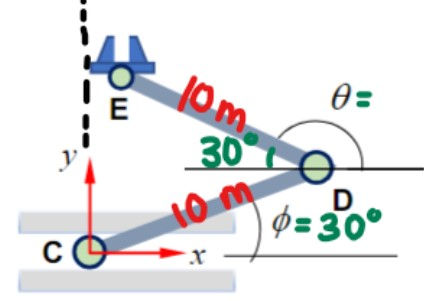
\includegraphics[width=0.3\textwidth]{figure3.jpg}
    \caption{Geometrical Diagram of System}
    \label{fig:label2}
\end{figure}

\FloatBarrier

To solve for the variable $\phi$ for MATLAB implementation, the total distance in the y-direction for the base arm is used and calculated. The value of $\phi$ is ignored where it is defined, though through geometry the inner angle is equal to 30 degrees. It is then written in terms of x. 

\begin{align}
    y = 10sin\phi + 10sin30\degree \\ 
    \phi = sin^{-1}(\frac{y-10sin30\degree}{10}) \\ 
    \phi = sin^{-1}(\frac{(\sqrt{100-x})-10sin30\degree}{10})
\end{align}

Additionally, the values of $\dot\phi$ and $\ddot\phi$ can be found using the equations for $\vec{V_{Ey}}$ and $\vec{a_{Ey}}$. \\ 

Remembering the following relationships: 

\begin{align*}
    \vec{\omega_{CD}}=\dot\phi\hat{k}\\ \vec{a_{CD}}=\ddot\phi\hat{k}
\end{align*}

Solving for $\dot\phi$:

\begin{align*}
    \vec{V_{Ey}} = \dot\phi 10cos\phi \\ 
    \dot\phi = \frac{\vec{V_{Ey}}}{10 cos\phi}
\end{align*}
\begin{equation}
    \vec{\omega_{CD}} = \frac{\vec{V_{Ey}}}{10 cos\phi}
\end{equation}

Solving for $\ddot\phi$:

\begin{align*}
    \vec{a_{Ey}} = \ddot\phi 10cos\phi - \dot\phi^2 10sin\phi \\ 
    \ddot\phi = \frac{\vec{a_{Ey}}+\dot\phi^2 10sin\phi}{10cos\phi}
\end{align*}
\begin{equation}
    \vec{a_{CD}} = \frac{\vec{a_{Ey}}+(\vec{\omega_{CD}})^2 10sin\phi}{10cos\phi}
\end{equation}

The following code was used to create this simulation: \\ \\ \\ 

\begin{lstlisting}
    function [VEx,VEy,aEx,aEy,VCx,aCx,om_CD,alp_CD] = lab2;

% Students need to download NFCdata.txt from D2L and put in the folder 
% for numerical analysis of the capture.
%
% 1. There are 5000 rows and 7 columns in NFCdata.txt. The 7 columns are 
%    etx, ety, enx, eny, rho, t, s, respectively, where, for 0 <= x <= 20
% 2. etx,ety: (x,y) components of the tangential basis vector et, 
% 3. enx,eny: (x,y) components of the normal basis vector en, 
% 4. rho: radius of curvature ((1+y'^2)^1.5/|y''|) for, 
% 5. t: the time instants of NFC at location x, and
% 6. s: the arc length of travel along the flight path y = sqrt(100-x)

% Load NFCdata.txt and define coor and travel info of NFC

x = linspace(0,20,5000)';
y_NFC = sqrt(100-x);
nx = length(x);

load NFCdata.txt;

etx=NFCdata(:,1);
ety=NFCdata(:,2);
enx=NFCdata(:,3);
eny=NFCdata(:,4);
rho=NFCdata(:,5);
t=NFCdata(:,6);
s=NFCdata(:,7);

theta=150/180*pi;
V0_NFC = 4;
at_NFC = V0_NFC/t(end);

% NFC velocity, accel at location x of the capture zone

V_NFC = sqrt(16 - 2*at_NFC*s);   % TODO 1
VEx = V_NFC.*etx;
VEy = V_NFC.*ety;
an_NFC = V_NFC.^2./rho;          % TODO 2
aEx = at_NFC.*etx + an_NFC.*enx;
aEy = at_NFC.*ety + an_NFC.*eny;

% Calculate base arm kinematics: phi, om_CD
phi = asin((y_NFC-(10*sind(30)))/10);  % TODO 3 - phi
om_CD = VEy./(10*cos(phi));            % TODO 4 - phi dot 
alp_CD = (aEy+10*(om_CD.*om_CD)).*sin(phi)./(10*cos(phi));  % TODO 5 - phi double dot

% Calculate point C kinematics of the base arm movement: VCx, aCx

VCx = VEx+(10*om_CD.*sin(phi));     % TODO 6
aCx = aEx+(10.*alp_CD.*sin(phi))+(10*om_CD.*om_CD.*cos(phi));    % TODO 7

% (FIGURE 1): Plotting V_Ex vs. x
plot(x, VEx);
title('1. V_{Ex} vs. x');
xlabel('x');
ylabel('V_{Ex}');

% (FIGURE 2): Plotting V_Ey vs. x
plot(x, VEy);
title('2. V_{Ey} vs. x');
xlabel('x');
ylabel('V_{Ey}');

% (FIGURE 3): Plotting a_Ex vs. x
plot(x, aEx);
title('3. a_{Ex} vs. x');
xlabel('x');
ylabel('a_{Ex}');

% (FIGURE 4): Plotting a_Ey vs. x
plot(x, aEy);
title('4. a_{Ey} vs. x');
xlabel('x');
ylabel('a_{Ey}');

% (FIGURE 5): Plotting V_Cx vs. x
% plot(x, VCx);
% title('5. V_{Cx} vs. x');
% xlabel('x');
% ylabel('V_{Cx}');

% (FIGURE 6): Plotting a_Cx vs. x
plot(x, aCx);
title('6. a_{Cx} vs. x');
xlabel('x');
ylabel('a_{Cx}');

% (FIGURE 7): Plotting om_CD or theta' vs. x
plot(x, om_CD);
title('7. \omega_{CD} (theta.) vs. x');
xlabel('x');
ylabel('\omega_{CD}');

% (FIGURE 8): Plotting alp_CD (theta'') vs. x
plot(x, alp_CD);
title('8. \alpha_{CD} (theta..) vs. x');
xlabel('x');
ylabel('\alpha_{CD}');
\end{lstlisting}

\FloatBarrier

\newpage
\section{NUMERICAL RESULTS (Deliverable F Part 2)}

\textbf{Produce 8 plots: $V_{Ex}, V_{Ey}, a_{Ex}, a_{Ey}, V_{cx}, a_{cx}, \dot\phi, \ddot\phi$ as functions of x.}

\begin{figure}[htbp]
    \centering
    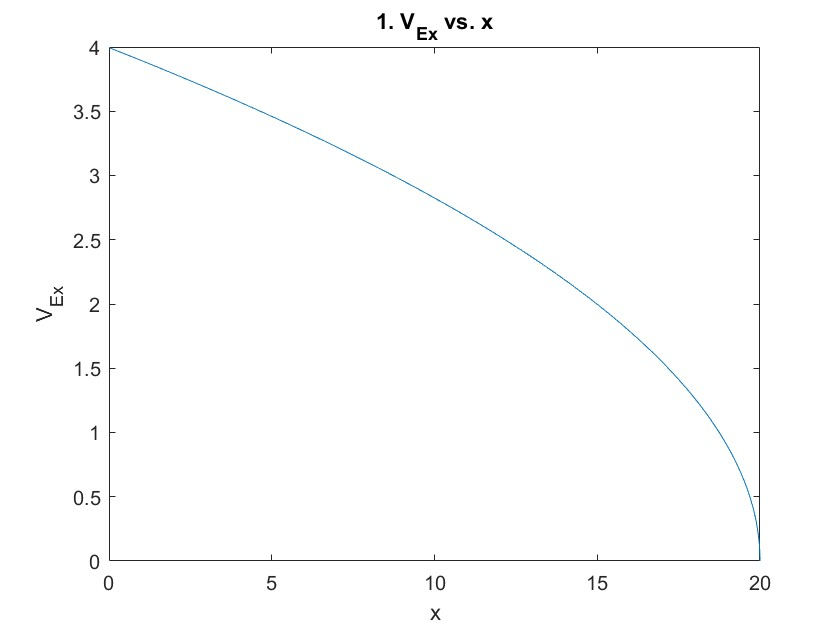
\includegraphics[width=0.6\textwidth]{graph1.jpg}
    \caption{$V_{Ex}$ vs $x$}
    \label{fig:label2}
\end{figure}

\FloatBarrier

\begin{figure}[htbp]
    \centering
    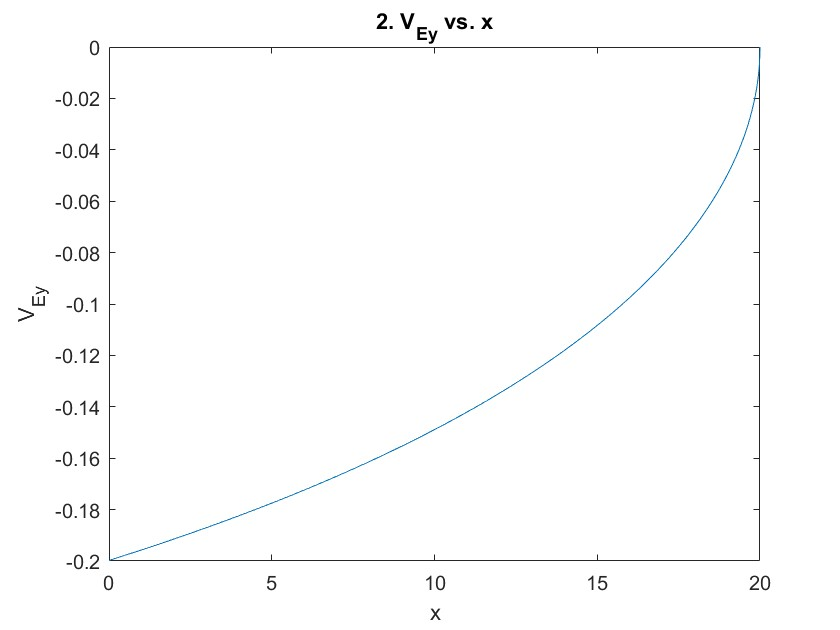
\includegraphics[width=0.6\textwidth]{graph2.jpg}
    \caption{$V_{Ey}$ vs $x$}
    \label{fig:label2}
\end{figure}

\FloatBarrier

\begin{figure}[htbp]
    \centering
    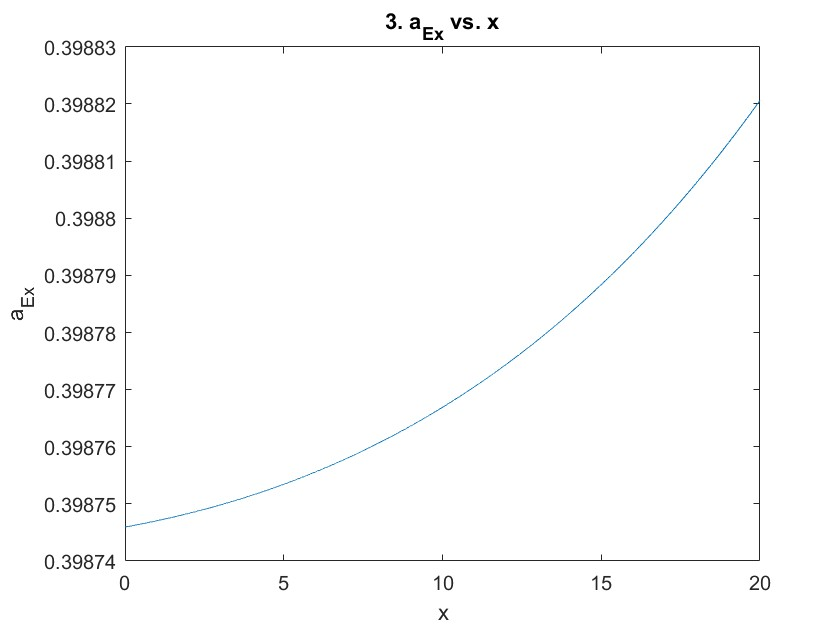
\includegraphics[width=0.6\textwidth]{graph3.jpg}
    \caption{$a_{Ex}$ vs $x$}
    \label{fig:label2}
\end{figure}

\FloatBarrier

\begin{figure}[htbp]
    \centering
    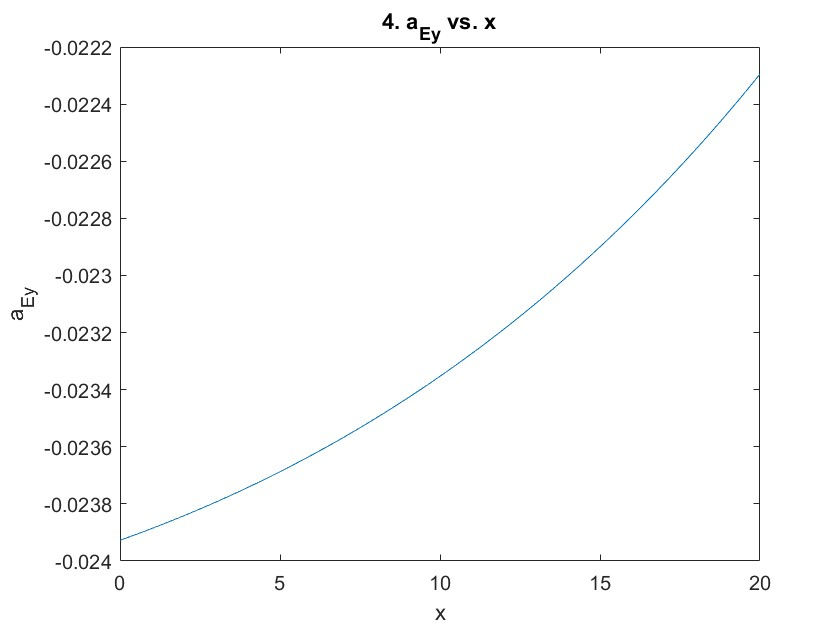
\includegraphics[width=0.6\textwidth]{graph4.jpg}
    \caption{$a_{Ey}$ vs $x$}
    \label{fig:label2}
\end{figure}

\FloatBarrier

\begin{figure}[htbp]
    \centering
    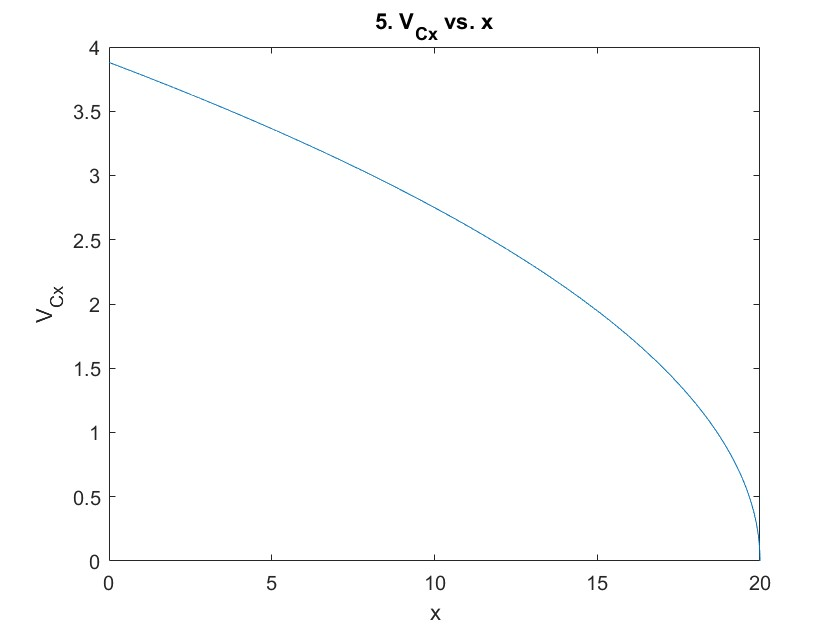
\includegraphics[width=0.6\textwidth]{graph5.jpg}
    \caption{$V_{Cx}$ vs $x$}
    \label{fig:label2}
\end{figure}

\FloatBarrier

\begin{figure}[htbp]
    \centering
    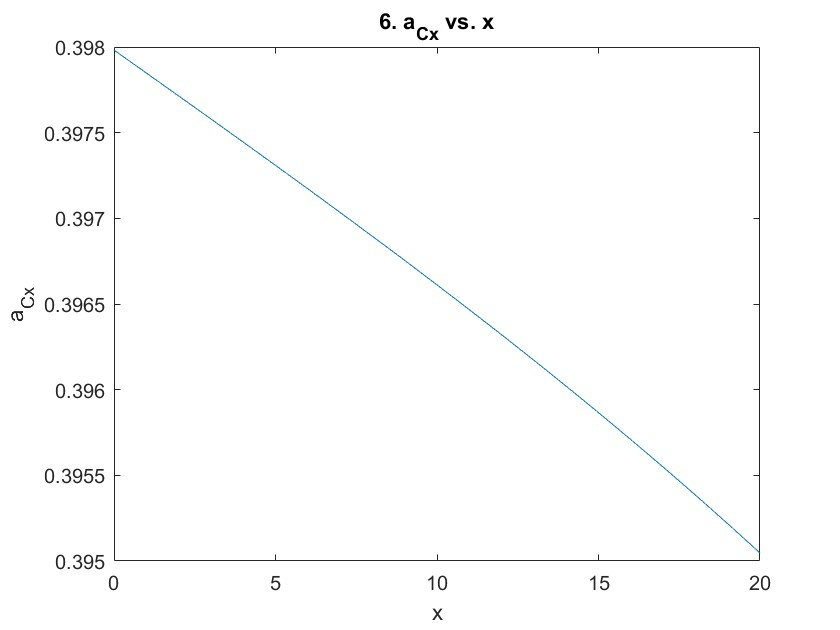
\includegraphics[width=0.6\textwidth]{graph6.jpg}
    \caption{$a_{Cx}$ vs $x$}
    \label{fig:label2}
\end{figure}

\FloatBarrier

\begin{figure}[htbp]
    \centering
    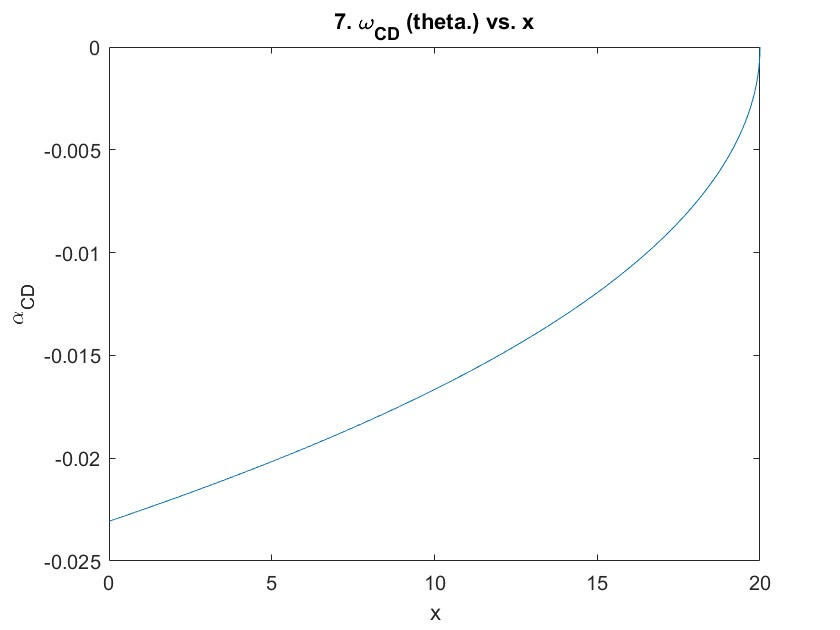
\includegraphics[width=0.6\textwidth]{graph7.jpg}
    \caption{$\omega_{CD} (\dot\theta)$ vs $x$}
    \label{fig:label2}
\end{figure}

\FloatBarrier

\begin{figure}[htbp]
    \centering
    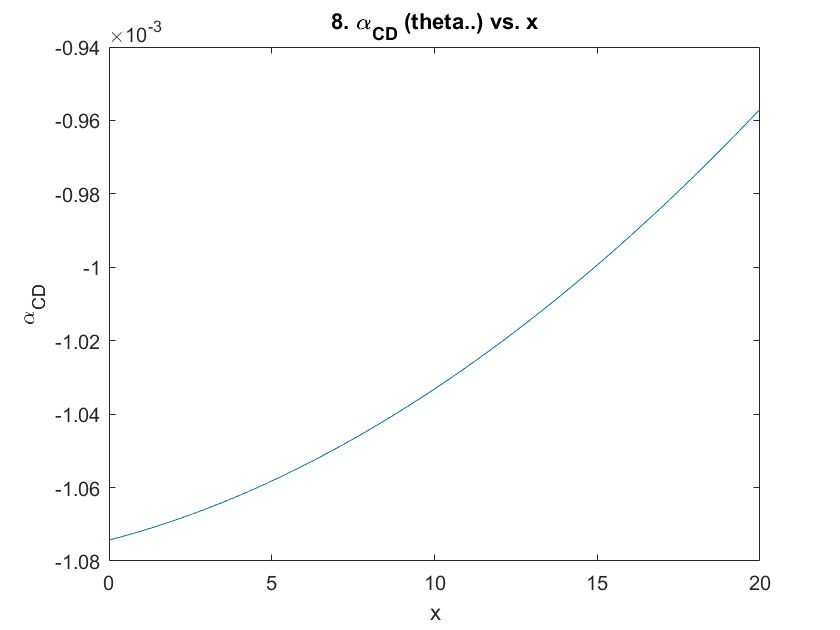
\includegraphics[width=0.6\textwidth]{graph8.jpg}
    \caption{$\alpha_{CD} (\ddot\theta)$ vs $x$}
    \label{fig:label2}
\end{figure}

\FloatBarrier

\end{document}